\documentclass[a4paper,12pt,titlepage]{article}
\usepackage{amsmath} 
\usepackage{amssymb}
\usepackage[nottoc]{tocbibind}
\usepackage{bm}
\usepackage{float}
\usepackage{indentfirst}
\usepackage{extarrows}
\author{\textit{Jiang Yicheng}\\\textit{515370910224}}
\title{\textbf{VE311 
		Note}}
\date{\today}
\usepackage{mathrsfs}
\usepackage[top=1 in, bottom=1 in, left= 1in, right=1 in]{geometry}
\usepackage{fancyhdr,lastpage}
	\pagestyle{fancy}
	\fancyhf{}
\lhead{VE414\\Assignment 1}
\rhead{Jiang Yicheng\\515370910224}
\cfoot{Page \thepage\ of \pageref{LastPage}}
\usepackage{multirow}
\usepackage{gauss}
\usepackage{graphicx}
\usepackage{dsfont}
\usepackage{enumerate}

\begin{document}


\section*{1.}
\subsection*{(a)}
Denote Narvey Dent picks up a double-headed coin as event ``DH", a double-tailed coin as event ``DT", and a normal one as ``N". Denote the lower face of the coin is a head as event ``LH". According to Bayes' theorem, 
\begin{align*}
    P[\text{LH}]=&P[\text{LH}|\text{DH}]P[\text{DH}]+P[\text{LH}|\text{DT}]P[\text{DT}]+P[\text{LH}|\text{N}]P[\text{N}]\\
    =&1\cdot\dfrac{2}{5}+0\cdot\dfrac{1}{5}+\dfrac{1}{2}\cdot\dfrac{2}{5}\\
    =&\dfrac{3}{5}
\end{align*}
So the probability is $\dfrac{3}{5}$.

\subsection*{(b)}
Denote the top face of the coin showing  heads as ``TH". Then,
\begin{align*}
    P[\text{LH}|\text{TH}]=&\dfrac{P[\text{TH}\cap\text{LH}]}{P[\text{TH}]}=\dfrac{P[\text{DH}]}{P[\text{TH}|\text{DH}]P[\text{DH}]+P[\text{TH}|\text{DT}]P[\text{DT}]+P[\text{TH}|\text{N}]P[\text{N}]}\\
    =&\dfrac{\dfrac{2}{5}}{1\cdot\dfrac{2}{5}+0+\dfrac{1}{2}\cdot\dfrac{2}{5}}\\
    =&\dfrac{2}{3}
\end{align*}
So the probability is $\dfrac{2}{3}$.

\subsection*{(c)}
After opening eyes, Harvey knows that this coin cannot be a double-tailed one. Then
\begin{align*}
    P[\text{LH}|\text{TH}]=&\dfrac{P[\text{TH}\cap\text{LH}]}{P[\text{TH}]}=\dfrac{P[\text{DH}]}{P[\text{TH}|\text{DH}]P[\text{DH}]+P[\text{TH}|\text{N}]P[\text{N}]}\\
    =&\dfrac{\dfrac{2}{4}}{1\cdot\dfrac{2}{4}+\dfrac{1}{2}\cdot\dfrac{2}{4}}\\
    =&\dfrac{2}{3}
\end{align*}
So the probability is $\dfrac{2}{3}$.

\section*{2.}
Denote $X_k$ as the number of heads' appearing out of $k$ number of trials, with the assumption of independence, then we have
$$X_k\sim Binomial (k; p)$$
and the likelihood function
$$\mathcal{L}(p; x) = f_{X|P} (x | p) =\dfrac{k!}{x!(k-x)!}p^x(1-p)^{k-x}$$
Then
\begin{align*}
    f_{P|x}(p)=\dfrac{f_{XP}(x,p)}{f_{X}(x)}=\dfrac{f_{X|P}(x|p)f_P(p)}{f_X(x)}\propto f_{X|P}(x|p)f_P(p)
\end{align*}
Given that $X_{10}<3$, $P\sim$Beta(4,4), we get that
\begin{align*}
    f_{P|x<3}(p)=&A\cdot\Big(f_{X|P}(0|p)+f_{X|P}(1|p)+f_{X|P}(2|p)\Big)f_{P}(p)\\
    =&A\cdot\Big(\dfrac{10!}{0!(10-0)!}p^0(1-p)^{(10-0)}+\dfrac{10!}{1!(10-1)!}p^1(1-p)^{(10-1)}\\
    &+\dfrac{10!}{2!(10-2)!}p^2(1-p)^{(10-2)}\Big)\dfrac{\Gamma(4+4)}{\Gamma(4)\Gamma(4)}p^{4-1}(1-p)^{(4-1)}\\
    =&A\cdot\Big(p^3(1-p)^{13}+10p^4(1-p)^{12}+45p^5(1-p)^{11}\Big)
\end{align*}
where $A$ is a scale constant. Since
\begin{align*}
    1=&\int_{0}^{1}f_{P|x<3}(p)\,\,dp\\
    =&A\cdot\Big(\dfrac{\Gamma(4)\Gamma(14)}{\Gamma(18)}+10\cdot\dfrac{\Gamma(5)\Gamma(13)}{\Gamma(18)}+45\cdot\dfrac{\Gamma(6)\Gamma(12)}{\Gamma(18)}\Big)\\
\end{align*}
the posterior density for $p$ is 
$$f_{P|x}(p)=\dfrac{7735}{8}(p^3(1-p)^{13}+10p^4(1-p)^{12}+45p^5(1-p)^{11})$$
\begin{figure}[H]
    \centering
    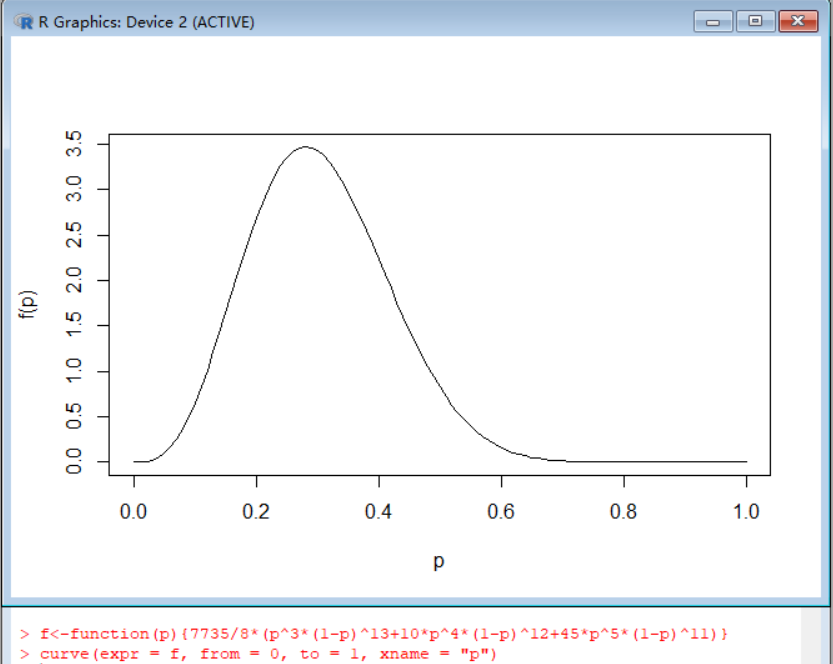
\includegraphics[scale=0.8]{2.PNG}
\end{figure}

\section*{3.}
Let $X_1$ denote the number of people choose ``$F$" is one test, and $X_2$ denote the number of people choose ``$J$''. Then $X_1+X_2=50$ and the probability of choosing either of items is the binomial distribution.  Assume that these people would like to choose $F$ with probability $p$ and $J$ with probability $1-p$. Then
$$f_{X_1X_2}(x_1, x_2)=\dfrac{50!}{x_1!x_2!}p^{x_1}(1-p)^{x_2}=\dfrac{50!}{y!(50-y)!}p^y(1-p)^{50-y}=:f_Y(y)$$

Given this binomial distribution, the likelihood function for parameter $p$ is
$$\mathcal{L}(p;y)=f_{Y_1|p}(y_1|p)f_{Y_2|p}(y_2|p)=\dfrac{50!50!}{y_1!(50-y_1)!y_2!(50-y_2)!}p^{y_1+y_2}(1-p)^{50-y_1+50-y_2}$$
Assume a uniform prior $f_P(p)=\left\{
\begin{aligned}
1\,\,\,,\,&0<p<1\\
0\,\,\,,\,&\text{otherwise}\\
\end{aligned}
\right.$, then the posterior of $p$ is
\begin{align*}
    f_{P|y_1,y_2}(p)=&A\cdot p^{y_1+y_2}(1-p)^{100-(y_1+y_2)}f_{P}(p)=\left\{
\begin{aligned}
A\cdot p^{y_1+y_2}(1-p)^{100-(y_1+y_2)}\,\,\,,\,&0<p<1\\
0\quad\quad\quad\quad\quad\,\,\,,\,&\text{otherwise}\\
\end{aligned}
\right.
\end{align*}
where $A$ is a scale constant. Since $y_1=40$, $y_2=15$, and
\begin{align*}
    1=&\int_{-\infty}^{\infty}f_{P}(p)\,\,dp=\int_{0}^{1}p^{55}(1-p)^{45}\,\,dp\\
    =&\dfrac{\Gamma(56)\Gamma(46)}{\Gamma(102)}
\end{align*}
$A=\dfrac{\Gamma(102)}{\Gamma(56)\Gamma(46)}$. Then the posterior mean is given by
\begin{align*}
    \hat{p}=&\mathbb{E}[P]=\int_{-\infty}^{\infty}pf_{P}(p)\,\,dp=A\cdot\int_{0}^{1}pp^{55}(1-p)^{45}\,\,dp\\
     =&A\cdot\int_{0}^{1}p^{56}(1-p)^{45}\,\,dp=\dfrac{\Gamma(102)}{\Gamma(56)\Gamma(46)}\dfrac{\Gamma(57)\Gamma(46)}{\Gamma(103)}\\
     =&\dfrac{56}{102}>\dfrac{1}{2}
\end{align*}
So $\hat{p}=\dfrac{1}{2}$ and therefore it seems that people are biased toward $F$.



\section*{4.}
\subsection*{(a)}
Given the geometric distribution with PDF
$$f_{X_i|p}(x_i | p) = p(1 - p)^{x_i-1}$$
the likelihood function for parameter $p$ is
$$\mathcal{L}(p;x)=\prod\limits_{i=1}^nf_{X_i|p}(x_i | p)=p^n(1 - p)^{\sum\limits_{i=1}^nx_i-n}$$
and we can obtain that
\begin{align*}
    &\dfrac{d\, \mathcal{L}(p;x)}{dp}=np^{n-1}(1-p)^{\sum\limits_{i=1}^nx_i-n}-(\sum\limits_{i=1}^nx_i-n)p^n(1-p)^{\sum\limits_{i=1}^nx_i-n-1}\\
\end{align*}
So
$$\dfrac{d\, \mathcal{L}(p;x)}{dp}=0\Leftrightarrow n(1-p)=(\sum\limits_{i=1}^nx_i-n)p\Leftrightarrow p=\dfrac{n}{\sum\limits_{i=1}^nx_i}$$
Since 
$$\lim_{p\searrow0+}\mathcal{L}(p;x)\rightarrow0<\mathcal{L}(\dfrac{1}{\bar{x}};x)$$
$\mathcal{L}(p;x_i)$ reaches its maximum at $p=\dfrac{1}{\bar{x}}$, i.e. $\widetilde{p}=\dfrac{1}{\bar{x}}$.

\subsection*{(b)}
For $p\in(0,\dfrac{1}{2})$, $p=\varphi(q)=\dfrac{1-\sqrt{1-4q}}{2}\Rightarrow \dfrac{d\,\varphi(q)}{d\,q}=\dfrac{1}{\sqrt{1-4q}}>0$.
Then
\begin{align*}
    \dfrac{d\, \mathcal{L}(\varphi(q);x)}{dq}=0&\Leftrightarrow \dfrac{d\, \mathcal{L}(\varphi(q);x)}{d\varphi(q)}\dfrac{d\,\varphi(q)}{d\,q}=0 \\
    &\Leftrightarrow \dfrac{d\, \mathcal{L}(\varphi(q);x)}{d\varphi(q)}=0\\
    &\Leftrightarrow \varphi(q)=\dfrac{n}{\sum\limits_{i=1}^nx_i}=\dfrac{1}{\bar{x}}
\end{align*}
which is valid for $\bar{x}>2$, and $q=\dfrac{\bar{x}-1}{\bar{x}^2}$, $\mathcal{L}(\varphi(q);x)=\dfrac{1}{\bar{x}^n}(1-\dfrac{1}{\bar{x}})^{n\bar{x}-n}=\dfrac{(\bar{x}-1)^{n\bar{x}-n}}{\bar{x}^{n\bar{x}}}$.

Similarly, for $p\in(\dfrac{1}{2}, 1)$, $p=\varphi(q)=\dfrac{1+\sqrt{1-4q}}{2}\Rightarrow \dfrac{d\,\varphi(q)}{d\,q}=-\dfrac{1}{\sqrt{1-4q}}<0$, then
$$\varphi(q)=\dfrac{1}{\bar{x}}$$
which is valid for $1<\bar{x}<2$  and $q=\dfrac{\bar{x}-1}{\bar{x}^2}$, $\mathcal{L}(\varphi(q);x)=\dfrac{(\bar{x}-1)^{n\bar{x}-n}}{\bar{x}^{n\bar{x}}}$.

For $q=\dfrac{1}{4}$, we have $p=\dfrac{1}{2}$, $\varphi(q)=\dfrac{1}{\bar{x}}$ which is valid when $\bar{x}=2$.

Finally, if $\bar{x}=1$, then $x_i=1$ and $\mathcal{L}(p;x)=p^n$ reaches maximum when $p\rightarrow1$ and therefore $q\rightarrow0$.
So $\hat{q}=\dfrac{\bar{x}-1}{\bar{x}^2}$.
%And if $$ \mathcal{L}(\dfrac{1}{2};x)=\dfrac{1}{2^n}\cdot\dfrac{1}{2^{n\bar{x}-n}}=\dfrac{1}{2^{n\bar{x}}}$$ is the maximum, we would find that 

\subsection*{(c)}
Given the uniform prior $f_P(p)=\left\{
\begin{aligned}
1\,\,\,,\,&0<p<1\\
0\,\,\,,\,&\text{otherwise}\\
\end{aligned}
\right.$, and the likelihood for parameter $p$,
\begin{align*}
    \mathcal{L}(p;x)=\prod\limits_{i=1}^nf_{X_i|p}(x_i | p)=p^n(1 - p)^{\sum\limits_{i=1}^nx_i-n}=(p(1-p)^{\bar{x}-1})^n
\end{align*}
then the posterior of $p$ is
\begin{align*}
    f_{P|\bar{x}}(p)=&A\cdot (p(1-p)^{\bar{x}-1})^nf_{P}(p)=\left\{
\begin{aligned}
A\cdot(p(1-p)^{\bar{x}-1})^n\,\,\,,\,&0<p<1\\
0\quad\quad\quad\quad\quad\,\,\,,\,&\text{otherwise}\\
\end{aligned}
\right.
\end{align*}
where $A$ is a scale constant. Since 
\begin{align*}
    1=&\int_{-\infty}^{\infty}f_{P|\bar{x}}(p)\,\,dp=\int_{0}^{1}(p(1-p)^{\bar{x}-1})^n\,\,dp\\
    =&\int_{0}^{1}p^{n+1-1}(1-p)^{n\bar{x}-n+1-1}\,\,dp\\
    =&\dfrac{\Gamma(n+1)\Gamma(n\bar{x}-n+1)}{\Gamma(n\bar{x}+2)}
\end{align*}
$A=\dfrac{\Gamma(n\bar{x}+2)}{\Gamma(n+1)\Gamma(n\bar{x}-n+1)}$. Then the posterior mean is given by
\begin{align*}
    \hat{p}=&\mathbb{E}[P]=\int_{-\infty}^{\infty}pf_{P|\bar{x}}(p)\,\,dp=A\cdot\int_{0}^{1}p(p(1-p)^{\bar{x}-1})^n\,\,dp\\
     =&A\cdot\int_{0}^{1}p^{n+2-1}(1-p)^{n\bar{x}-n+1-1}\,\,dp=\dfrac{\Gamma(n\bar{x}+2)}{\Gamma(n+1)\Gamma(n\bar{x}-n+1)}\dfrac{\Gamma(n+2)\Gamma(n\bar{x}-n+1)}{\Gamma(n\bar{x}+3)}\\
     =&\dfrac{n+1}{n\bar{x}+2}
\end{align*}
So $\hat{p}=\dfrac{n+1}{n\bar{x}+2}$.


\end{document}